\documentclass[conference]{IEEEtran}


% *** GRAPHICS RELATED PACKAGES ***
%
\ifCLASSINFOpdf
\usepackage{graphicx}
  % declare the path(s) where your graphic files are
  %\graphicspath{{../pdf/}{../jpeg/}}
  % and their extensions so you won't have to specify these with
  % every instance of \includegraphics
\DeclareGraphicsExtensions{.pdf,.jpeg,.png}
\else
  % or other class option (dvipsone, dvipdf, if not using dvips). graphicx
  % will default to the driver specified in the system graphics.cfg if no
  % driver is specified.
\usepackage[dvips]{graphicx}
  % declare the path(s) where your graphic files are
  %\graphicspath{{../eps/}}
  % and their extensions so you won't have to specify these with
  % every instance of \includegraphics
\DeclareGraphicsExtensions{.eps}
\fi
% graphicx was written by David Carlisle and Sebastian Rahtz. It is
% required if you want graphics, photos, etc. graphicx.sty is already
% installed on most LaTeX systems. The latest version and documentation can
% be obtained at:
% http://www.ctan.org/tex-archive/macros/latex/required/graphics/
% Another good source of documentation is "Using Imported Graphics in
% LaTeX2e" by Keith Reckdahl which can be found as epslatex.ps or
% epslatex.pdf at: http://www.ctan.org/tex-archive/info/
%
% latex, and pdflatex in dvi mode, support graphics in encapsulated
% postscript (.eps) format. pdflatex in pdf mode supports graphics
% in .pdf, .jpeg, .png and .mps (metapost) formats. Users should ensure
% that all non-photo figures use a vector format (.eps, .pdf, .mps) and
% not a bitmapped formats (.jpeg, .png). IEEE frowns on bitmapped formats
% which can result in "jaggedy"/blurry rendering of lines and letters as
% well as large increases in file sizes.
%
% You can find documentation about the pdfTeX application at:
% http://www.tug.org/applications/pdftex





% *** MATH PACKAGES ***
%
\usepackage[cmex10]{amsmath}
\newtheorem{IEEEdef}{Definition}
\newtheorem{IEEEthe}{Theorem}
\newtheorem{IEEEcor}{corollary}
% A popular package from the American Mathematical Society that provides
% many useful and powerful commands for dealing with mathematics. If using
% it, be sure to load this package with the cmex10 option to ensure that
% only type 1 fonts will utilized at all point sizes. Without this option,
% it is possible that some math symbols, particularly those within
% footnotes, will be rendered in bitmap form which will result in a
% document that can not be IEEE Xplore compliant!
%
% Also, note that the amsmath package sets \interdisplaylinepenalty to 10000
% thus preventing page breaks from occurring within multiline equations. Use:
%\interdisplaylinepenalty=2500
% after loading amsmath to restore such page breaks as IEEEtran.cls normally
% does. amsmath.sty is already installed on most LaTeX systems. The latest
% version and documentation can be obtained at:
% http://www.ctan.org/tex-archive/macros/latex/required/amslatex/math/





% *** SPECIALIZED LIST PACKAGES ***
%
\usepackage{algorithmic}
% algorithmic.sty was written by Peter Williams and Rogerio Brito.
% This package provides an algorithmic environment fo describing algorithms.
% You can use the algorithmic environment in-text or within a figure
% environment to provide for a floating algorithm. Do NOT use the algorithm
% floating environment provided by algorithm.sty (by the same authors) or
% algorithm2e.sty (by Christophe Fiorio) as IEEE does not use dedicated
% algorithm float types and packages that provide these will not provide
% correct IEEE style captions. The latest version and documentation of
% algorithmic.sty can be obtained at:
% http://www.ctan.org/tex-archive/macros/latex/contrib/algorithms/
% There is also a support site at:
% http://algorithms.berlios.de/index.html
% Also of interest may be the (relatively newer and more customizable)
% algorithmicx.sty package by Szasz Janos:
% http://www.ctan.org/tex-archive/macros/latex/contrib/algorithmicx/




% *** ALIGNMENT PACKAGES ***
%
%\usepackage{array}
% Frank Mittelbach's and David Carlisle's array.sty patches and improves
% the standard LaTeX2e array and tabular environments to provide better
% appearance and additional user controls. As the default LaTeX2e table
% generation code is lacking to the point of almost being broken with
% respect to the quality of the end results, all users are strongly
% advised to use an enhanced (at the very least that provided by array.sty)
% set of table tools. array.sty is already installed on most systems. The
% latest version and documentation can be obtained at:
% http://www.ctan.org/tex-archive/macros/latex/required/tools/


%\usepackage{mdwmath}
%\usepackage{mdwtab}
% Also highly recommended is Mark Wooding's extremely powerful MDW tools,
% especially mdwmath.sty and mdwtab.sty which are used to format equations
% and tables, respectively. The MDWtools set is already installed on most
% LaTeX systems. The lastest version and documentation is available at:
% http://www.ctan.org/tex-archive/macros/latex/contrib/mdwtools/


% IEEEtran contains the IEEEeqnarray family of commands that can be used to
% generate multiline equations as well as matrices, tables, etc., of high
% quality.


%\usepackage{eqparbox}
% Also of notable interest is Scott Pakin's eqparbox package for creating
% (automatically sized) equal width boxes - aka "natural width parboxes".
% Available at:
% http://www.ctan.org/tex-archive/macros/latex/contrib/eqparbox/





% *** SUBFIGURE PACKAGES ***
\usepackage[tight,footnotesize]{subfigure}
% subfigure.sty was written by Steven Douglas Cochran. This package makes it
% easy to put subfigures in your figures. e.g., "Figure 1a and 1b". For IEEE
% work, it is a good idea to load it with the tight package option to reduce
% the amount of white space around the subfigures. subfigure.sty is already
% installed on most LaTeX systems. The latest version and documentation can
% be obtained at:
% http://www.ctan.org/tex-archive/obsolete/macros/latex/contrib/subfigure/
% subfigure.sty has been superceeded by subfig.sty.



%\usepackage[caption=false]{caption}
%\usepackage[font=footnotesize]{subfig}
% subfig.sty, also written by Steven Douglas Cochran, is the modern
% replacement for subfigure.sty. However, subfig.sty requires and
% automatically loads Axel Sommerfeldt's caption.sty which will override
% IEEEtran.cls handling of captions and this will result in nonIEEE style
% figure/table captions. To prevent this problem, be sure and preload
% caption.sty with its "caption=false" package option. This is will preserve
% IEEEtran.cls handing of captions. Version 1.3 (2005/06/28) and later
% (recommended due to many improvements over 1.2) of subfig.sty supports
% the caption=false option directly:
%\usepackage[caption=false,font=footnotesize]{subfig}
%
% The latest version and documentation can be obtained at:
% http://www.ctan.org/tex-archive/macros/latex/contrib/subfig/
% The latest version and documentation of caption.sty can be obtained at:
% http://www.ctan.org/tex-archive/macros/latex/contrib/caption/

\usepackage[linesnumbered,ruled,vlined]{algorithm2e}


% *** FLOAT PACKAGES ***
%
%\usepackage{fixltx2e}
% fixltx2e, the successor to the earlier fix2col.sty, was written by
% Frank Mittelbach and David Carlisle. This package corrects a few problems
% in the LaTeX2e kernel, the most notable of which is that in current
% LaTeX2e releases, the ordering of single and double column floats is not
% guaranteed to be preserved. Thus, an unpatched LaTeX2e can allow a
% single column figure to be placed prior to an earlier double column
% figure. The latest version and documentation can be found at:
% http://www.ctan.org/tex-archive/macros/latex/base/



%\usepackage{stfloats}
% stfloats.sty was written by Sigitas Tolusis. This package gives LaTeX2e
% the ability to do double column floats at the bottom of the page as well
% as the top. (e.g., "\begin{figure*}[!b]" is not normally possible in
% LaTeX2e). It also provides a command:
%\fnbelowfloat
% to enable the placement of footnotes below bottom floats (the standard
% LaTeX2e kernel puts them above bottom floats). This is an invasive package
% which rewrites many portions of the LaTeX2e float routines. It may not work
% with other packages that modify the LaTeX2e float routines. The latest
% version and documentation can be obtained at:
% http://www.ctan.org/tex-archive/macros/latex/contrib/sttools/
% Documentation is contained in the stfloats.sty comments as well as in the
% presfull.pdf file. Do not use the stfloats baselinefloat ability as IEEE
% does not allow \baselineskip to stretch. Authors submitting work to the
% IEEE should note that IEEE rarely uses double column equations and
% that authors should try to avoid such use. Do not be tempted to use the
% cuted.sty or midfloat.sty packages (also by Sigitas Tolusis) as IEEE does
% not format its papers in such ways.


% *** PDF, URL AND HYPERLINK PACKAGES ***
%
%\usepackage{url}
% url.sty was written by Donald Arseneau. It provides better support for
% handling and breaking URLs. url.sty is already installed on most LaTeX
% systems. The latest version can be obtained at:
% http://www.ctan.org/tex-archive/macros/latex/contrib/misc/
% Read the url.sty source comments for usage information. Basically,
% \url{my_url_here}.





% *** Do not adjust lengths that control margins, column widths, etc. ***
% *** Do not use packages that alter fonts (such as pslatex).         ***
% There should be no need to do such things with IEEEtran.cls V1.6 and later.
% (Unless specifically asked to do so by the journal or conference you plan
% to submit to, of course. )


% correct bad hyphenation here
\hyphenation{op-tical net-works semi-conduc-tor}


\begin{document}
%
% paper title
% can use linebreaks \\ within to get better formatting as desired
\title{Mining High Utility Itemsets over Uncertain Databases}

\author{\IEEEauthorblockN{
    Yuqing Lan$^\dag$  \qquad
	Yang Wang$^\dag$   \qquad
	Yanni Wang$^\ddag$  \qquad
	Shengwei Yi$^\S$ \qquad
	Dan Yu$^\ast$
}
\IEEEauthorblockA{$^\dag$School of Computer Science and Engineering, Beihang University, Beijing, China\\
$^\ddag$School of Software, Beihang University, Beijing, China\\
$^\S$China Information Technology Security Evaluation Center, Beijing, China\\
$^\ast$China Standard Software Co. Ltd, Beijing, China\\
$^\dag$\{lanyuqing, yangwang\}@buaa.edu.cn, \quad
$^\ddag$wangyn@buaa.edu.cn, \quad
$^\S$yishengwei@foxmail.com, \quad
$^\ast$yudan@cs2c.com.cn
}}

% conference papers do not typically use \thanks and this command
% is locked out in conference mode. If really needed, such as for
% the acknowledgment of grants, issue a \IEEEoverridecommandlockouts
% after \documentclass

% for over three affiliations, or if they all won't fit within the width
% of the page, use this alternative format:
%
%\author{\IEEEauthorblockN{Michael Shell\IEEEauthorrefmark{1},
%Homer Simpson\IEEEauthorrefmark{2},
%James Kirk\IEEEauthorrefmark{3},
%Montgomery Scott\IEEEauthorrefmark{3} and
%Eldon Tyrell\IEEEauthorrefmark{4}}
%\IEEEauthorblockA{\IEEEauthorrefmark{1}School of Electrical and Computer Engineering\\
%Georgia Institute of Technology,
%Atlanta, Georgia 30332--0250\\ Email: see http://www.michaelshell.org/contact.html}
%\IEEEauthorblockA{\IEEEauthorrefmark{2}Twentieth Century Fox, Springfield, USA\\
%Email: homer@thesimpsons.com}
%\IEEEauthorblockA{\IEEEauthorrefmark{3}Starfleet Academy, San Francisco, California 96678-2391\\
%Telephone: (800) 555--1212, Fax: (888) 555--1212}
%\IEEEauthorblockA{\IEEEauthorrefmark{4}Tyrell Inc., 123 Replicant Street, Los Angeles, California 90210--4321}}




% use for special paper notices
%\IEEEspecialpapernotice{(Invited Paper)}




% make the title area
\maketitle


\begin{abstract}
%\boldmath
Recently, with the growing popularity of Internet of Things (IoT) and pervasive computing, a large amount of uncertain data, i.e. RFID data, sensor data, real-time monitoring data, etc., has been collected. As one of the most fundamental issues of uncertain data mining, the problem of mining uncertain frequent itemsets has attracted much attention in the database and data mining communities. Although some efficient approaches of mining uncertain frequent itemsets have been proposed, most of them only consider each item in one transaction as a random variable and ignore the utility of each item in the real scenarios. In this paper, we focus on the problem of mining high utility itemsets (MHUI) over uncertain databases, in which each item has a utility. In order to solve the MHUI problem over uncertain databases, we propose an efficient mining algorithm, named UHUI-apriori. Extensive experiments on both real and synthetic datasets verify the effectiveness and efficiency of our proposed solutions.
\end{abstract}
% IEEEtran.cls defaults to using nonbold math in the Abstract.
% This preserves the distinction between vectors and scalars. However,
% if the conference you are submitting to favors bold math in the abstract,
% then you can use LaTeX's standard command \boldmath at the very start
% of the abstract to achieve this. Many IEEE journals/conferences frown on
% math in the abstract anyway.

% no keywords




% For peer review papers, you can put extra information on the cover
% page as needed:
% \ifCLASSOPTIONpeerreview
% \begin{center} \bfseries EDICS Category: 3-BBND \end{center}
% \fi
%
% For peerreview papers, this IEEEtran command inserts a page break and
% creates the second title. It will be ignored for other modes.
\IEEEpeerreviewmaketitle



\section{Introduction}
Recently, with the growing popularity of Internet of Things (IoT) and pervasive computing, a large amount of uncertain data has been collected from different kinds of devices, such as RFID, sensors, and real-time monitoring systems\cite{tong2015tracking,tong2015mining}. As one of the most fundamental issues of uncertain data mining, the problem of mining uncertain frequent itemsets has attracted much attention in the database and data mining communities\cite{chui2007mining,aggarwal2009frequent,tong2012discovering,bernecker2009probabilistic,tong2012ufimt}. Although some efficient approaches of mining uncertain frequent itemsets have been proposed\cite{tong2012mining}, most of them only consider each item in one transaction as a random variable and ignore the unit utilities of items in the real scenarios.

In kinds of recommender system (e.g. music, video) analysis, mining frequent itemsets from an uncertain database refers to the discovery of itemsets which may frequently appear together in the records (transactions). However, in these works, the unit values (utilities) of items are not considered in their frameworks of uncertain frequent itemsets mining. Hence, it cannot satisfy the requirement of a user who is interested in discovering itemsets with high enjoyment values. For example, a table shows some songs and their utility values. The utility value of each song is scored by all the persons listened to it according to their preference degree to the song. Another is the listening records of some users showing which songs they listened to and the probability they like them. Namely, in a song transaction of a user, the probability he likes these songs are 0.8, 0.8, 0.7, and 0.7.When songs are recommended, not only the frequency of songs in records of different user should be considered, but the popularity of songs should also be taken into account. In view of this, utility mining is a necessary topic in data mining for discovering itemsets with high utility, such as values (utilities), in uncertain databases.

Mining high utility itemsets from the databases refers to finding the itemsets with high utilities\cite{chan2003mining,ahmed2009efficient,tseng2010up}. The basic meaning of utility is the interestingness / importance / profitability of an item to the users.

\vspace{-0.1cm}
\subsubsection*{To sum up, we make the following contributions:}

\begin{itemize}
\vspace{-0.2cm}
\item	To the best of our knowledge, this is the first work to formulate the problem of mining high utility itemsets over uncertain databases (MHUI).
\item   Due to the challenges from utility constraints, the downward closure could not be directly used to mine HUIs, we propose the UHUI-Apriori algorithm to mine HUIs.
\item   We verify the effectiveness and efficiency of the proposed methods through extensive experiments on real and synthetic datasets.
\vspace{-0.2cm}
\end{itemize}

The rest of the paper is organized as follows. Problem statement are introduced in Section 2. In Section 3, we present an efficient mining algorithm, named UHUI-Apriori. In Section 4, experimental evaluation on both real and synthetic datasets are reported. Finally, we conclude this paper in Section 5.


%\subsubsection{Subsubsection Heading Here}
%Subsubsection text here.


% An example of a floating figure using the graphicx package.
% Note that \label must occur AFTER (or within) \caption.
% For figures, \caption should occur after the \includegraphics.
% Note that IEEEtran v1.7 and later has special internal code that
% is designed to preserve the operation of \label within \caption
% even when the captionsoff option is in effect. However, because
% of issues like this, it may be the safest practice to put all your
% \label just after \caption rather than within \caption{}.
%
% Reminder: the "draftcls" or "draftclsnofoot", not "draft", class
% option should be used if it is desired that the figures are to be
% displayed while in draft mode.
%
%\begin{figure}[!t]
%\centering
%\includegraphics[width=2.5in]{myfigure}
% where an .eps filename suffix will be assumed under latex,
% and a .pdf suffix will be assumed for pdflatex; or what has been declared
% via \DeclareGraphicsExtensions.
%\caption{Simulation Results}
%\label{fig_sim}
%\end{figure}

% Note that IEEE typically puts floats only at the top, even when this
% results in a large percentage of a column being occupied by floats.


% An example of a double column floating figure using two subfigures.
% (The subfig.sty package must be loaded for this to work.)
% The subfigure \label commands are set within each subfloat command, the
% \label for the overall figure must come after \caption.
% \hfil must be used as a separator to get equal spacing.
% The subfigure.sty package works much the same way, except \subfigure is
% used instead of \subfloat.
%
%\begin{figure*}[!t]
%\centerline{\subfloat[Case I]\includegraphics[width=2.5in]{subfigcase1}%
%\label{fig_first_case}}
%\hfil
%\subfloat[Case II]{\includegraphics[width=2.5in]{subfigcase2}%
%\label{fig_second_case}}}
%\caption{Simulation results}
%\label{fig_sim}
%\end{figure*}
%
% Note that often IEEE papers with subfigures do not employ subfigure
% captions (using the optional argument to \subfloat), but instead will
% reference/describe all of them (a), (b), etc., within the main caption.


% An example of a floating table. Note that, for IEEE style tables, the
% \caption command should come BEFORE the table. Table text will default to
% \footnotesize as IEEE normally uses this smaller font for tables.
% The \label must come after \caption as always.
%
%\begin{table}[!t]
%% increase table row spacing, adjust to taste
%\renewcommand{\arraystretch}{1.3}
% if using array.sty, it might be a good idea to tweak the value of
% \extrarowheight as needed to properly center the text within the cells
%\caption{An Example of a Table}
%\label{table_example}
%\centering
%% Some packages, such as MDW tools, offer better commands for making tables
%% than the plain LaTeX2e tabular which is used here.
%\begin{tabular}{|c||c|}
%\hline
%One & Two\\
%\hline
%Three & Four\\
%\hline
%\end{tabular}
%\end{table}


% Note that IEEE does not put floats in the very first column - or typically
% anywhere on the first page for that matter. Also, in-text middle ("here")
% positioning is not used. Most IEEE journals/conferences use top floats
% exclusively. Note that, LaTeX2e, unlike IEEE journals/conferences, places
% footnotes above bottom floats. This can be corrected via the \fnbelowfloat
% command of the stfloats package.



\section{Problem Statement}
In this section, we give several basic definitions about mining high utility itemsets from uncertain data.

Let $I =\{i_1,i_2,...,i_n\}$ be a set of distinct items. Each item $i_p$ has a unit value $u(i_p)$. We name a non-empty subset, $X$, of $I$ as an itemset. For brevity, we use $X = x_1x_2...x_n$ to denote itemset $X = \{x_1,x_2,...x_n\}$. $X$ is a $l$ - item set if it has $l$ items. Given an uncertain transaction database $D$, each transaction is denoted as $< tid, Y >$, where $tid$ is the transaction identifier, and $Y = \{y_1(p_1),y_2(p_2),...,y_m(p_m)\}$. $Y$ contains $m$ units. Each unit has an item $y_i$ and probability $p_i$, denoting the possibility of item $y_i$ appearing in the $tid$ tuple. A threshold, the minimum utility threshold, is defined as $\mu$.

An example of uncertain databases is shown in Table 1. The corresponding utility table is shown in Table 2. In this example, the minimum utility threshold is set at $\mu$ (= 25\%).



\begin{IEEEdef}
\label{def:UI}
The utility of an item $i_j$ in $T_d$ is defined as:
\end{IEEEdef}

\vspace{-0.5cm}
\begin{equation}
\label{eq:UI}
U(i_j, T_d) =
p(i_j, T_d) \times u(i_j)
\end{equation}
\vspace{-0.5cm}

For example, the utility of an item (A) in $T_1$ is $U(A, T_1)= p(A, T_1) \times u(A) = 0.2 \times 4 = 0.8$ .

\begin{IEEEdef}
\label{def:UX}
The utility of an itemset $X$ in transaction $T_d$ is denoted as $U(X, T_d)$, which can be defined as:
\end{IEEEdef}

\vspace{-0.4cm}
\begin{equation}
\label{eq:UX}
U(X,T_d)
= \sum_{i_j \in X \wedge X \subseteq T_d}
U(i_j, T_d)
\end{equation}
\vspace{-0.4cm}

For example, the utility of (AC) in $T_1$ is calculated as $U(AC, T_1) = U(A, T_1) + U(C, T_1) = p(A, T_1) \times u(A) + p(C, T_1) \times u(C) = (0.2 \times 4) + (0.3 \times 12)$ = 4.4.

\begin{table}
  \centering
  \caption{An Uncertain Database}
  \label{tab:UD}
  \begin{tabular}{|c|l|}\hline
  \bfseries {TID} & \bfseries {Transactions} \\ \hline
  $T_1$ & A (0.2) C (0.3) E (0.2) \\ \hline
  $T_2$ & B (0.2) D (0.3) \\ \hline
  $T_3$ & A (0.1) B (0.2) C (0.1) E (0.3) \\ \hline
  $T_4$ & C (0.2) \\ \hline
  $T_5$ & B (0.3) D (0.2) E (0.1) \\ \hline
  $T_6$ & A (0.2) C (0.2) D (0.5) \\ \hline
  $T_7$ & A (0.1) B (0.1) D (0.4) E (0.1) \\ \hline
  $T_8$ & B (0.4) E (0.1) \\ \hline
  $T_9$ & A (0.3) C (0.3) D (0.2) \\ \hline
  $T_{10}$ & B (0.2) C (0.3) E (0.1) \\ \hline
  \end{tabular}
\end{table}

\begin{table}
  \centering
  \caption{An Utility Table}
  \label{tab:UT}
  \begin{tabular}{|c|c|c|c|c|c|}\hline
  \bfseries {TID} & \bfseries {A} & \bfseries {B} & \bfseries {C} & \bfseries {D} & \bfseries {E} \\ \hline
  Utility & 4 & 1 & 12 & 6 & 15\\ \hline
  \end{tabular}
\end{table}

\begin{IEEEdef}
\label{def:U}
The utility of an itemset $X$ in Uncertain database $D$ is denoted as $U(X)$, which can be defined as:
\end{IEEEdef}

\vspace{-0.4cm}
\begin{equation}
\label{eq:U}
U(X)
= \sum_{X \subseteq T_d \wedge T_d \in D}
U(X,T_d)
\end{equation}
\vspace{-0.4cm}

For example,  $U(A) = U(A, T_1) + U(A, T_3) + U(A, T_6) + U(A, T_7) + U(A, T_8) = (0.8 + 0.4 + 0.8 + 0.4 + 1.2)$ = 3.6, and $U(AC) = U(AC, T_1) + U(AC, T_3) + U(AC, T_6) + U(AC, T_9) = (4.4 + 1.6 + 3.2 + 4.8)$ = 14.

\begin{IEEEdef}
\label{def:TU}
The transaction utility of transaction $T_q$ is denoted as $tu(T_q)$, which can be defined as:
\end{IEEEdef}

\vspace{-0.4cm}
\begin{equation}
\label{eq:TU}
tu(T_q)
= \sum_{j=1}^{m}
U(i_j,T_d)
\end{equation}
\vspace{-0.4cm}

in which $m$ is the number of items in $T_d$.

For example, $TU(T_1) = U(A, T_1) + U(C, T_1) + U(E, T_1)$ = 0.8 + 3.6 + 3 = 7.4.

\begin{IEEEdef}
\label{def:DU}
The total utility in $D$ is the sum of all transaction utilities in D and is denoted as TU, which can be defined as:
\end{IEEEdef}

\vspace{-0.4cm}
\begin{equation}
\label{eq:DU}
TU
= \sum_{T_d \in D}
TU(T_d)
\end{equation}
\vspace{-0.4cm}

For example, the transaction utilities for $T_1$ to $T_{10}$ are respectively calculated as $TU(T_1)$ = 7.4, $TU(T_2)$ = 1.3, $TU(T_3)$ = 6.3, $TU(T_4)$ = 2.4, $TU(T_5)$ = 3, $TU(T_6)$ = 6.2, $TU(T_7)$ = 4.4, $TU(T_8)$ = 1.9, $TU(T_9)$ = 6.0, $TU(T_{10})$ = 5.3. The total utility in $D$ is the sum of all transaction utilities in $D$, which is calculated as: $TU$ = (7.4 + 1.3 + 6.3 + 2.4 + 3 + 6.2 + 4.4 + 1.9 + 6 + 5.3) = 44.2.

\begin{IEEEdef}
\label{def:HUI}
An itemset X is defined as a high utility itemset (HUI) if its utility value U(X) is not less than the minimum utility count as:
\end{IEEEdef}

\vspace{-0.4cm}
\begin{equation}
\label{eq:HUI}
\sum_{X \subseteq T_d \wedge T_d \in D}U(X,T_d)
= U(X) \geq \mu \times TU
\end{equation}
\vspace{-0.4cm}

For example, suppose that the minimum utility threshold $\mu$ is set at 25\%. An item (A) is not considered as a HUI since U(A) = 3.6, which is smaller than $(0.25 \times 44.2) = 11.05$. An itemset(AC) is considered as a HUI in D since U(AC) = 14, which is larger than the minimum utility count = 11.05.

Based on the above definitions, the problem statement of mining HUIs over uncertain databases can be formulated as follows:

Given an uncertain database D with total utility is $TU$, the minimum utility threshold which is set as $\mu$. The problem of MHUI over uncertain databases is to mine HUIs whose utilities are not less than ($\mu \times TU$).

From the example given in Tables 1 and Table 2, the set of HUIs is shown in Table 3 when the minimum utility threshold is set at $\mu = 25\%$.

\begin{table}
  \centering
  \caption{Derived HUIs over an uncertain database}
  \label{tab:HUIs}
  \begin{tabular}{|c|c|}\hline
  \bfseries Itemset & \bfseries Actual Utility \\ \hline
  (C) & 16.8 \\ \hline
  (E) & 13.5 \\ \hline
  (AC) & 14 \\ \hline
  (BE) & 11.7 \\ \hline
  (CE) & 17.4 \\ \hline
  (ACD) & 12.2 \\ \hline
  (ACE) & 13.5 \\ \hline
  \end{tabular}
\end{table}

\section{Proposed a Mining High Utility Itemsets Algorithm over Uncertain Databases}

To the best of our knowledge, this is the first paper to discuss the MHUI over uncertain databases. In this section, we propose the UHUI-apriori algorithm to mine HUIs over uncertain databases.

\vspace{-0.1cm}
\subsection{Pruning strategy by downward closure property}

In the well-known Apriori algorithm, the downward closure (DC) property is kept to reduce the number of candidates for association-rule mining (ARM). The DC property is also kept in the designed UHUI-apriori algorithm for mining HUIs. In MUHI over uncertain databases, the DC property of ARM could not be directly extended to mine HUIs. The transaction-weighted downward closure (TWDC) property was proposed to reduce the search space in MHUI.

\begin{IEEEdef}
\label{def:TWU}
The transaction-weighted utility (TWU) of an itemset X is the sum of all transaction utilities $TU(T_d)$ containing an itemset X, which is defined as:
\end{IEEEdef}

\vspace{-0.4cm}
\begin{equation}
\label{def:TWU}
TWU(X)
= \sum_{X \subseteq T_d \wedge T_d \in D}
TU(T_d)
\end{equation}
\vspace{-0.4cm}

\begin{IEEEdef}
\label{def:HTWUI}
An itemset X is considered as a high transaction-weighted utilization itemset (HTWUI) if its $TWU(X) \geq TU \times \mu$.
\end{IEEEdef}

In Table 1, the TWU of an item (E) is calculated as $TWU(E) = TU(T_1) + TU(T_3) + TU(T_5) + TU(T_7) + TU(T_8) + TU(T_{10})$ = (74 + 63 + 30 + 44 + 19 + 53) = 283. An item (E) is considered as a HTWUI since $TWU(E) = 283 \geq 134$.

\begin{IEEEthe}[Downward Closure Property of HTWUI]
\label{the:DC}
Let $X^k$ and $X^{k-1}$ be the HTWUI from uncertain databases, and $X^{k-1} \subseteq X^k$. The $TWU(X^{k-1}) \geq TWU(X^k)$.
\end{IEEEthe}

\begin{proof}
\label{pro:DC}
Let $X^{k-1}$ be a (k-1)-itemset and its superset k-itemset is denoted as $X^k$. Since $X^{k-1} \subseteq X^k$, thus,

\vspace{-0.7cm}
{\setlength\arraycolsep{1pt}
\small
\begin{eqnarray}
\label{eq:DC}
\ & TWU(X^k) & = \sum_{X^k\subseteq T_d\wedge T_d\in D}TU(T_d) {}
\nonumber \\
&&{} \leq \sum_{X^{k-1}\subseteq T_d\wedge T_d\in D}TU(T_d) {}
\nonumber \\
&&{} = TWU(X^{k-1}).
\end{eqnarray}}
\vspace{-1.2cm}

\end{proof}

\begin{IEEEcor}
\label{cor:sub}
If an itemset $X^k$ is a HTWUI, every subset $X^{k-1}$ of $X^k$ is a HTWUI.
\end{IEEEcor}

\begin{IEEEcor}
\label{cor:super}
If an itemset $X^k$ is not a HTWUI, no superset $X^{k+1}$ of $X^k$ is a HTWUI.
\end{IEEEcor}

\begin{IEEEthe}[HUIs $\subseteq$ HTWUIs]
\label{the:IN}
The transaction-weighted downward closure(TWDC) property ensures that HUIs $\subseteq$ HTWUIs, which indicates that if an itemset is not a HTWUI, then none of its supersets will be HUIs.
\end{IEEEthe}

\begin{proof}
\label{pro:IN}
$\forall X \subseteq D$, X is an itemset; thus,

\vspace{-0.7cm}
{\setlength\arraycolsep{1pt}
\small
\begin{eqnarray}
\label{eq:IN}
\ & U(X) & = \sum_{X\subseteq T_d\wedge T_d\in D}U(X, T_d) {}
\nonumber \\
&&{} \leq \sum_{X\subseteq T_d\wedge T_d\in D}TU(T_d) {}
\nonumber \\
&&{} = TWU(X).
\end{eqnarray}}
\vspace{-1.2cm}

\end{proof}

\vspace{-0.1cm}
\subsection{Detail of UHUI-apriori algorithm}

The proposed UHUI-apriori algorithms has two phases: in the first phase, the HTWUIs are found, and in the second phase, the HUIs are drived with an additional database rescan. The TWUDC property inherits the TWDC property of the two-phase model to keep the downward closure property, thus reducing the search space for finding HUIs. Only the remaining $HTWUI^{k-1}$ will be used to generate the next $C_k$ at each level. Based on the above definitions and theorems, detail of the proposed UHUI-apriori algorithm is described in UHUI-apriori algorithm.

Based on the designed TWUDC property, Theorem 2 ensures that the proposed UHUI-apriori algorithm can make sure that no supersets of small transaction-weighted itemsets are in the preliminary candidate set (correctness) and can extract the complete HUIs from the candidate HTWUIs (completeness). Therefore, the results of the proposed UHUI-apriori algorithm are correct and complete.

\begin{algorithm} %算法开始
\caption{Sample algorithm} %算法的题目
\label{alg1} %算法的标签
\begin{algorithmic}[1] %此处的[1]控制一下算法中的每句前面都有标号
\REQUIRE {$D$, an uncertain database; $utable$, utility table; $\mu$ minimum utility threshold;}
\ENSURE {the set of high utility itemsets (HUIs).}
\FOR{each $T_d$ in $D\wedge i_j$ in $T_d$}
\STATE calculate TWU($i_j$).
\ENDFOR
\FOR{each $T_d$ in $D\wedge i_j$ in $T_d$}
\IF{TWU($i_j$)$\geq TU \times \mu $}
\STATE  $HTWUI^1$ $\xleftarrow{}$ $i_j$.
\ENDIF
\ENDFOR
\STATE set $k \xleftarrow{} 2$.
\STATE set X as (k)-itemset.
\WHILE{$HTWUI^{k-1}\neq null$}
\STATE $C_k$ $\xleftarrow{}$ $Apriori_gen$($HTWUI^{k-1}$).
\FOR{each k-itemset X in $C_k$}
\STATE scan D to find TWU(X).
\IF{TWU(X)$\geq TU \times \mu$}
\STATE $HTWUI^k$ $\xleftarrow{}$ X.
\ENDIF
\ENDFOR
\STATE k $\xleftarrow{}$ K+1.
\ENDWHILE
\STATE HTWUIs $\xleftarrow{}$ $HTWUI^k$
\FOR{each k-itemset X in HTWUIs}
\STATE scan D to find u(X).
\IF {u(X)$\geq$ $TU \times \mu$}
\STATE $HUI^k$ $\xleftarrow{} X$.
\ENDIF
\ENDFOR
\STATE HUIs $\xleftarrow{}$ $HUI^k$.

\end{algorithmic}
\end{algorithm}

The proposed UHUI-apriori algorithm first scans the database to find the $TWU$ values and the probabilities of all 1-itemsets in database(Line 1 to 3). The set of $HTWUI^k$ (k is initially set as 1) is then produced (Lines 4 to 8) and will be further used to generate the next candidates $C_{K+1}$ for discovering $HTWUI^{k+1}$ in a level-wise way (Lines 11 to 20). In this process, the original database has to be rescanned to find the $HTWUI^{k+1}$ (Line 14). The first phase of UHUI-apriori algorithm is terminated when no candidate is generated. An additional database rescan is required in the second phase to find the final HUIs from the HTWUIs (Lines 22 to 29).

\vspace{-0.1cm}
\subsection{An illustrated example of UHUI-apriori algorithm}

In order to keep consistency, Tables 1 and 2 are used to illustrate the proposed UHUI-apriori algorithm as the example step-by-step. Assume the minimum utility threshold is also set at 25\%. The minimum support count can be calculated as $(44.2 \times 25\%)$ = 11.05. The UHUI-apriori algorithm first scans the database to find the TWU values of all 1-itemsets in the databases. The results are (A:30.3; B:22.2; C:33.6; D:20.9; E:28.3) in (A:30.3) indicates that the TWU(A) = 30.3. In this example, all itemsets satisfies the above conditions and then put into the set of $HTWUI^1$. Based on the designed UHUI-apriori algorithm, $C^2$ are then generated from $HTWUI^1$. A database scan is required to find the TWU values of $C^2$ as (AB:10.7; AC:25.9; AD:16.6; AE:18.1; BC:11.6; BD:8.7; BE:20.9; CD:12.2; CE:19; DE:7.4). Among them, only the itemsets (AC, AD, AE, BE, CD, CE) satisfy the condition as $TWU(X) \geq 11.05$; they are then put into the set of $HTWUI^2$. The variable $k$ is then set to 3. This process is repeated until no candidates are generated. The results are shown in Table 4.

\begin{table}
  \centering
  \caption{Derived HTWUIs over an uncertain database}
  \label{tab:HTHUIs}
  \begin{tabular}{|c|c|}\hline
  \bfseries Itemset & \bfseries TWU \\ \hline
  (A) & 30.3 \\ \hline
  (B) & 22.2 \\ \hline
  (C) & 33.6 \\ \hline
  (D) & 20.9 \\ \hline
  (E) & 28.3 \\ \hline
  (AC) & 25.9 \\ \hline
  (AD) & 16.6 \\ \hline
  (AE) & 18.1 \\ \hline
  (BE) & 20.9 \\ \hline
  (CD) & 12.2 \\ \hline
  (CE) & 19 \\ \hline
  (ACD) & 12.2 \\ \hline
  (ACE) & 13.7 \\ \hline
  \end{tabular}
\end{table}

After the first phase, the second phase is executed with an additional database scan to find the actual utility value of each remaining candidate. The results of HUIs were shown in Table 3.

\section{Experimental Evaluation}

Experiments for mining HUIs over uncertain datasets were conducted to evaluate the performance of the UHUI-apriori algorithm and the algorithm of direct traversal in terms of runtime, memory consumption. The algorithms in the experiments were implemented in C++ and performed on a PC with an Intel Core i5-3460 processor and 4GB of RAM. The platform is Visual Studio 2010 and 64-bit Microsoft Windows 7 OS. Experiments under varied minimum utility thresholds (MUs) is discussed below.

\vspace{-0.2cm}
\subsection{Datasets}

Both real-life and synthetic datasets were used in the experiments. A real-life datasets, namely accidents datasets, as well as one synthetic dataset, T10I4D100K, were used in the experiments to evaluate the performance of two algorithms. The utility values are assigned to the items in accidents and T10I4D100K datasets by simulation model. In addition, due to the tuple uncertainty property, each transaction in these datasets is assigned a unique probability value in the range of 0.1 to 0.5. The characteristics of used datasets are shown in Table 5.
\begin{figure}[htbp]
\vspace{-0.3cm}
  \centering
  \subfigure{
      \label{fig:time:ol}
      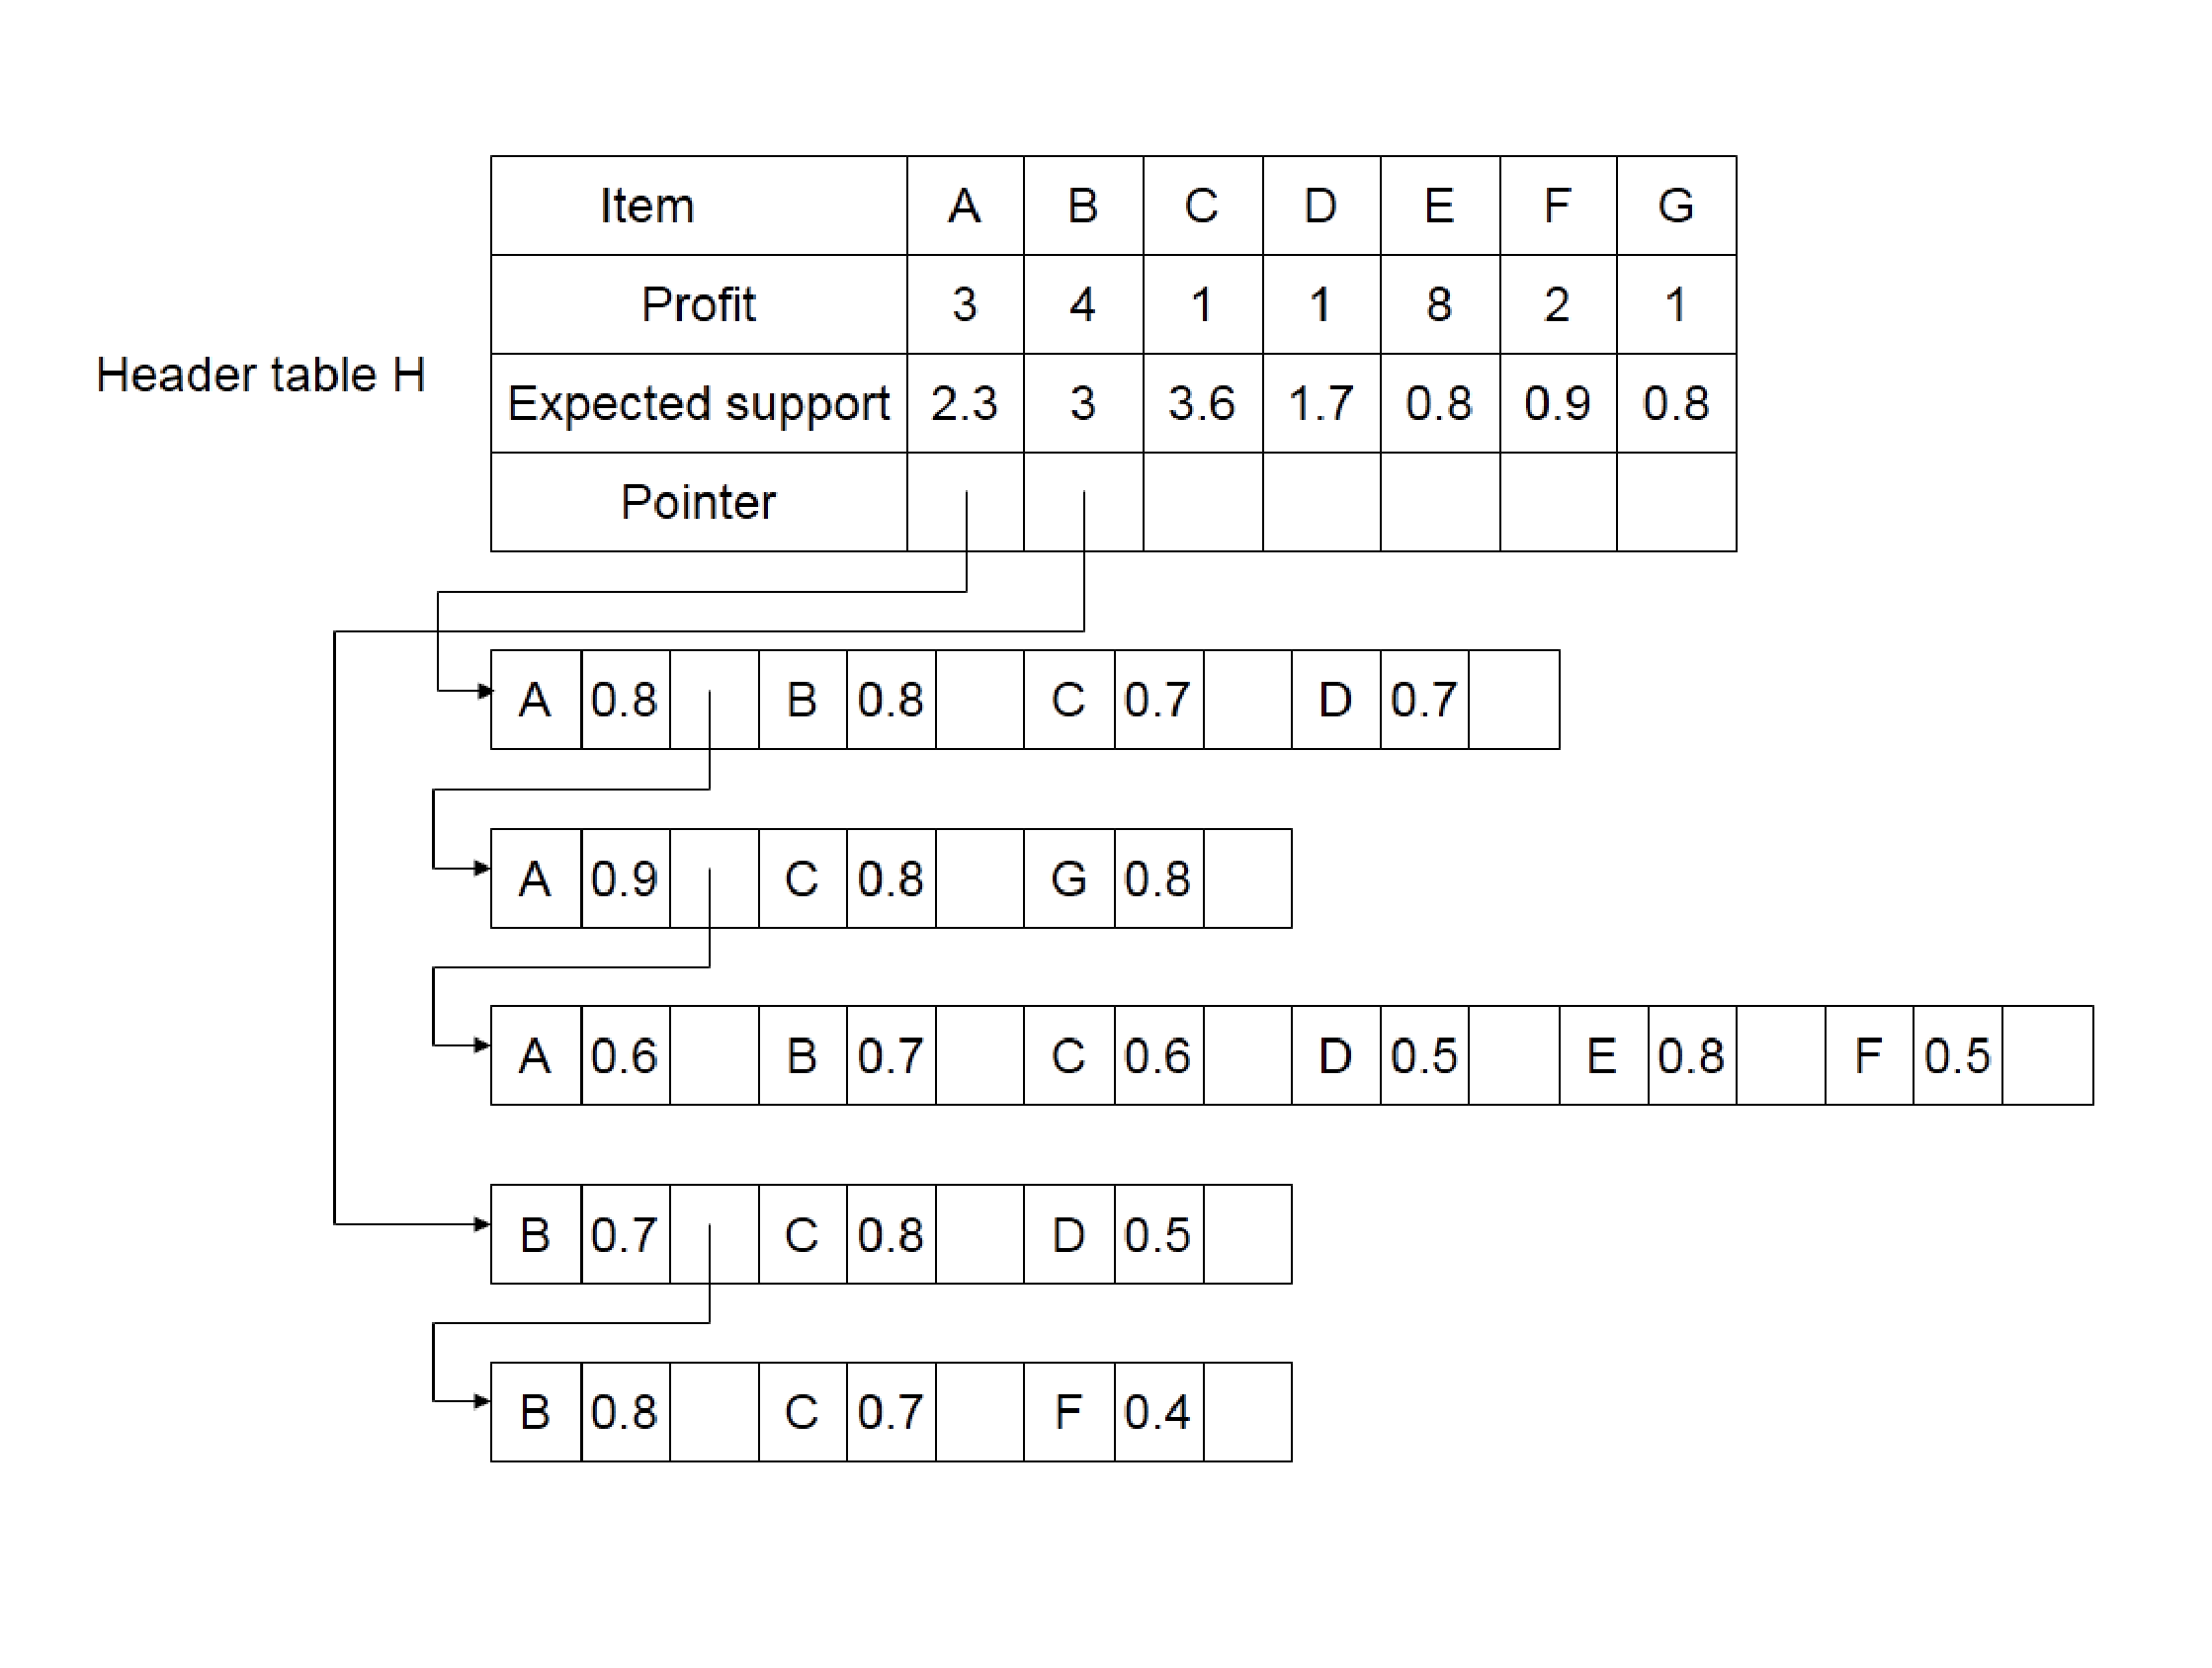
\includegraphics[width=0.23\textwidth]{1.eps}}
  \subfigure{
      \label{fig:time:sf}
      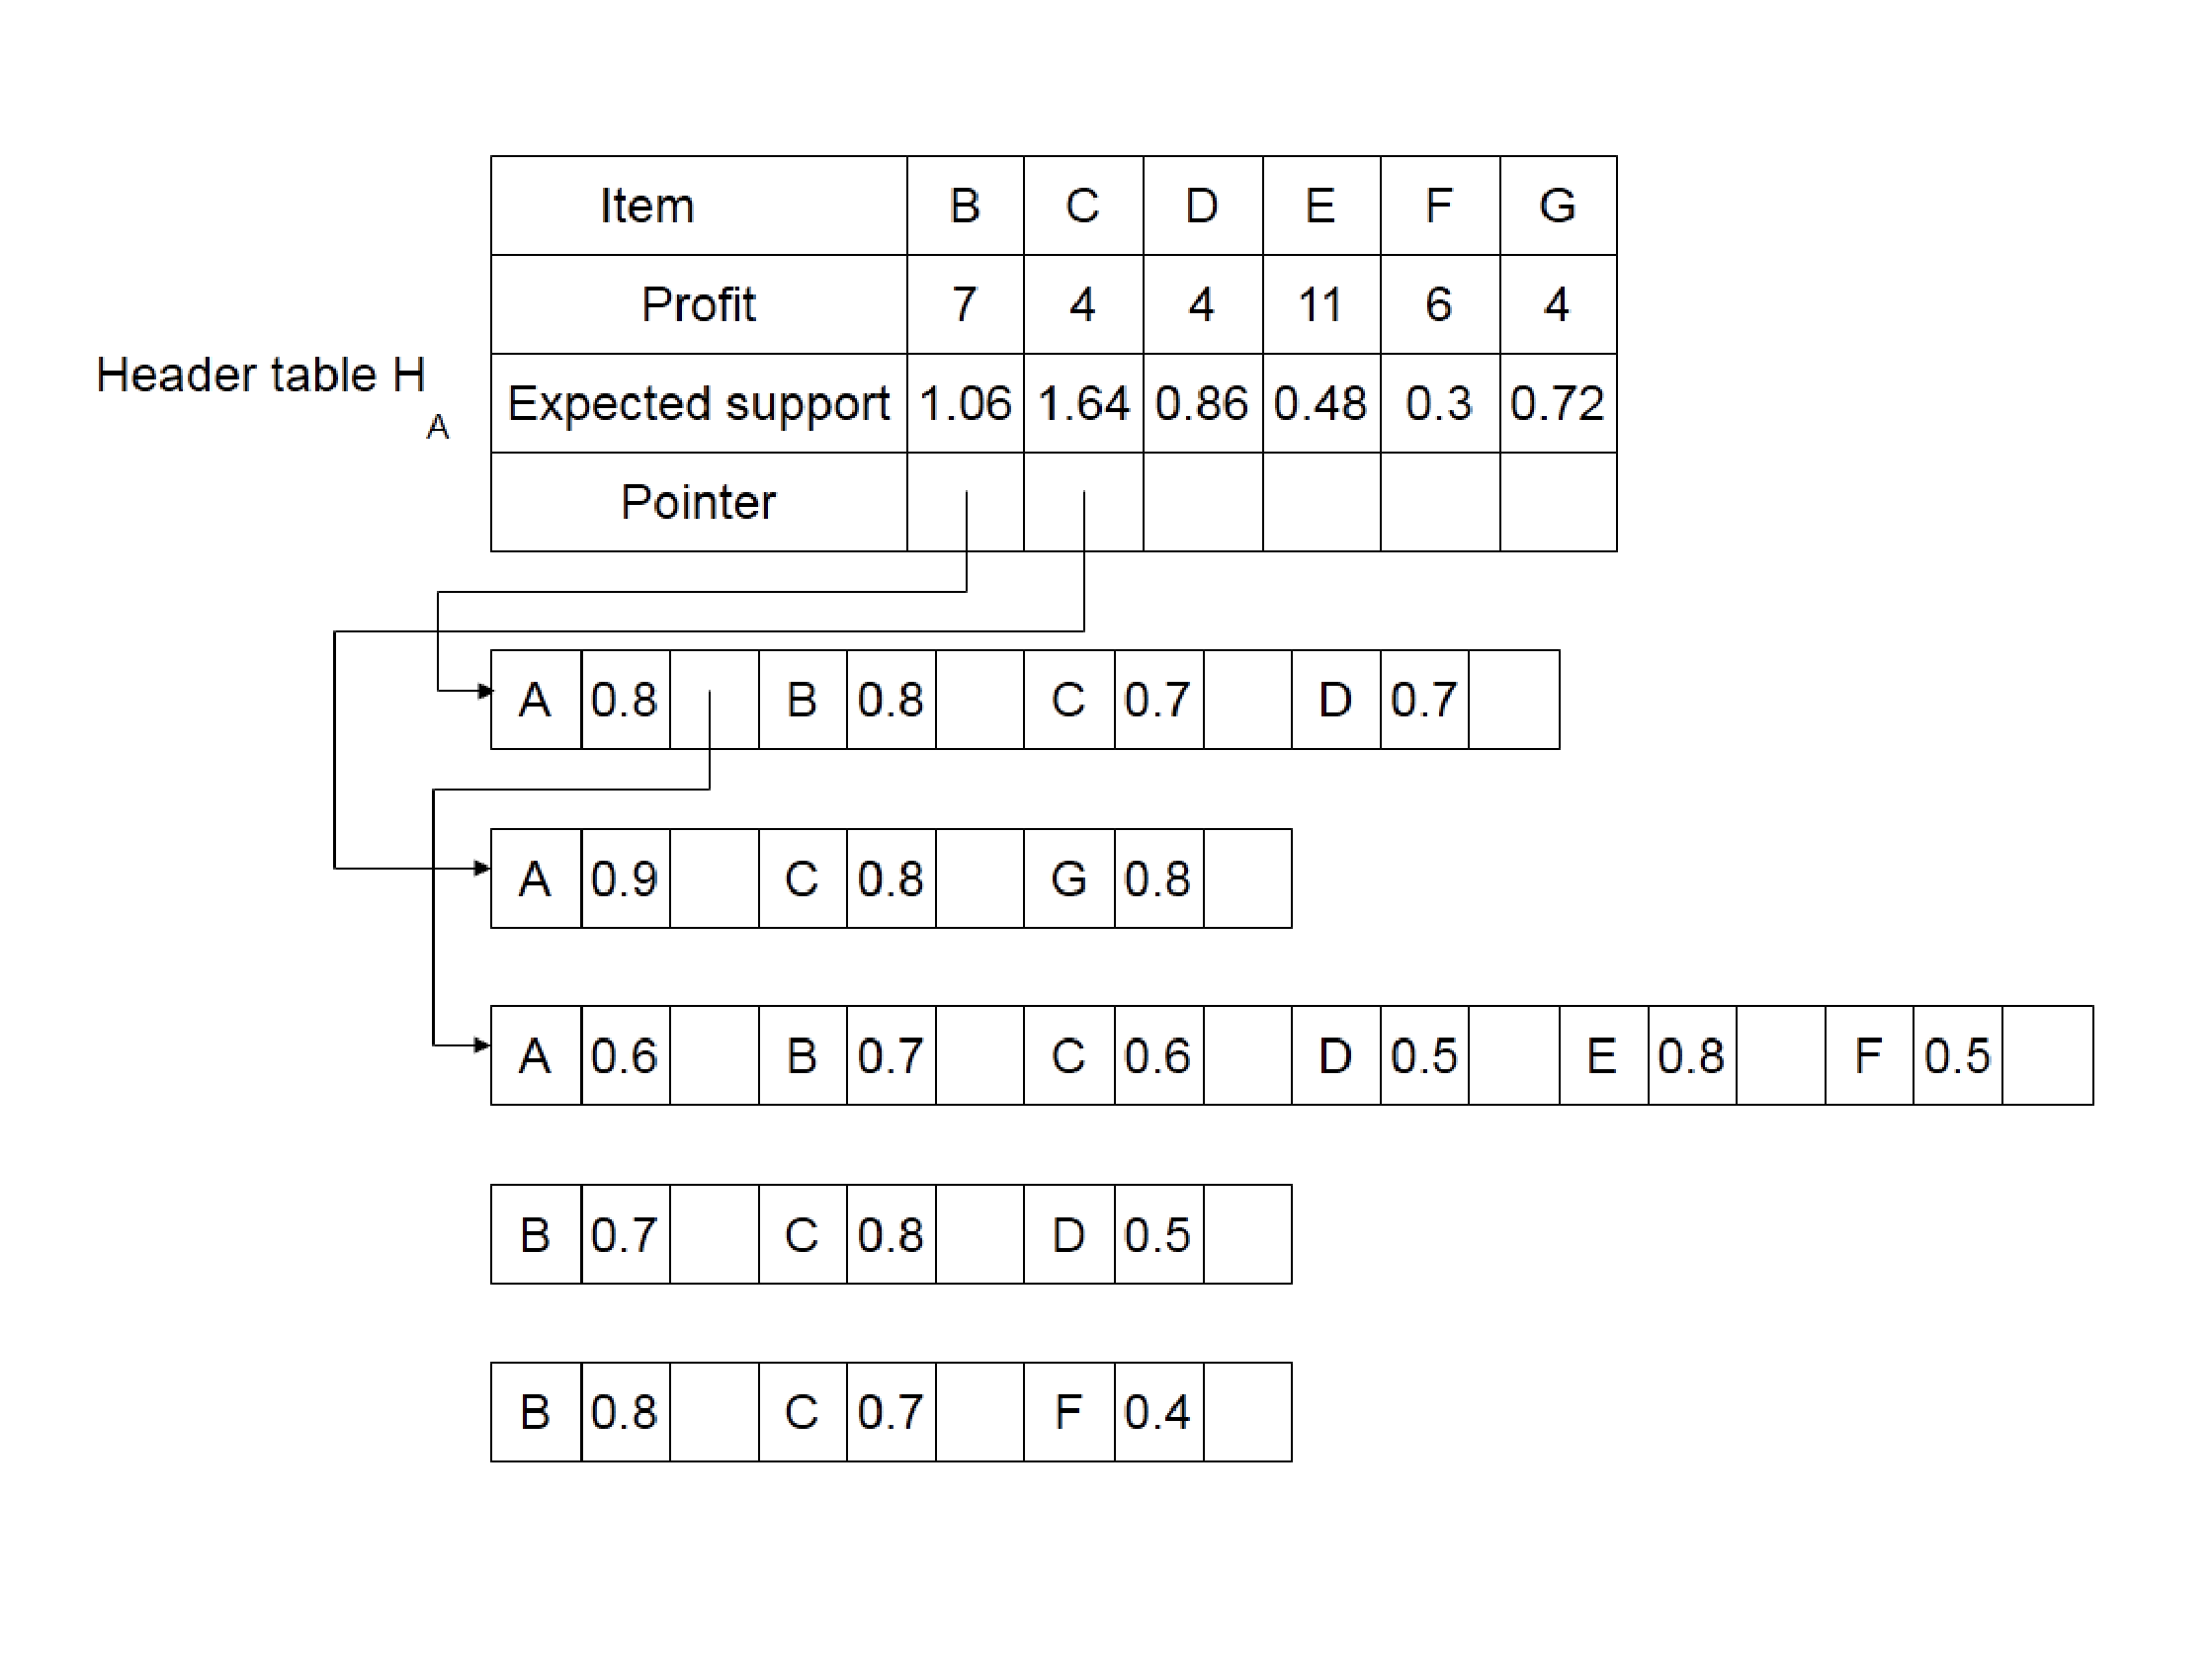
\includegraphics[width=0.23\textwidth]{2.eps}}
\vspace{-0.3cm}
  \caption{Runtime of two algorithms under varied MUs}
  \label{fig:time}
\vspace{-0.4cm}
\end{figure}

\begin{table}
  \centering
  \caption{Characteristics of used datasets}
  \label{tab:CUD}
  \begin{tabular}{|c|c|c|c|c|c|}\hline
  \bfseries {Database} & \bfseries {$|D|$} & \bfseries {$|I|$} & \bfseries {AvgLen} & \bfseries {MaxLen} & \bfseries {Type} \\ \hline
  accidents & 340,183 & 468 & 33.8 & 51 & dense\\ \hline
  T10I4D100K & 100,000 & 870 & 10.1 & 29 & sparse\\ \hline
  \end{tabular}
\end{table}

\vspace{-0.2cm}
\subsection{Runtime}

The runtime of the two algorithms under varied MUs are compared and shown in Fig.1.

From Fig.1, we can observe that the proposed UHUI-apriori algorithm has better performance than the algorithm of direct traversal.

\vspace{-0.2cm}
\subsection{Memory Consumption}

The memory consumption of the two algorithms under varied MUs are compared and shown in Fig.2.

\begin{figure}[htbp]
\vspace{-0.4cm}
  \centering
  \subfigure{
      \label{fig:memory:ol}
      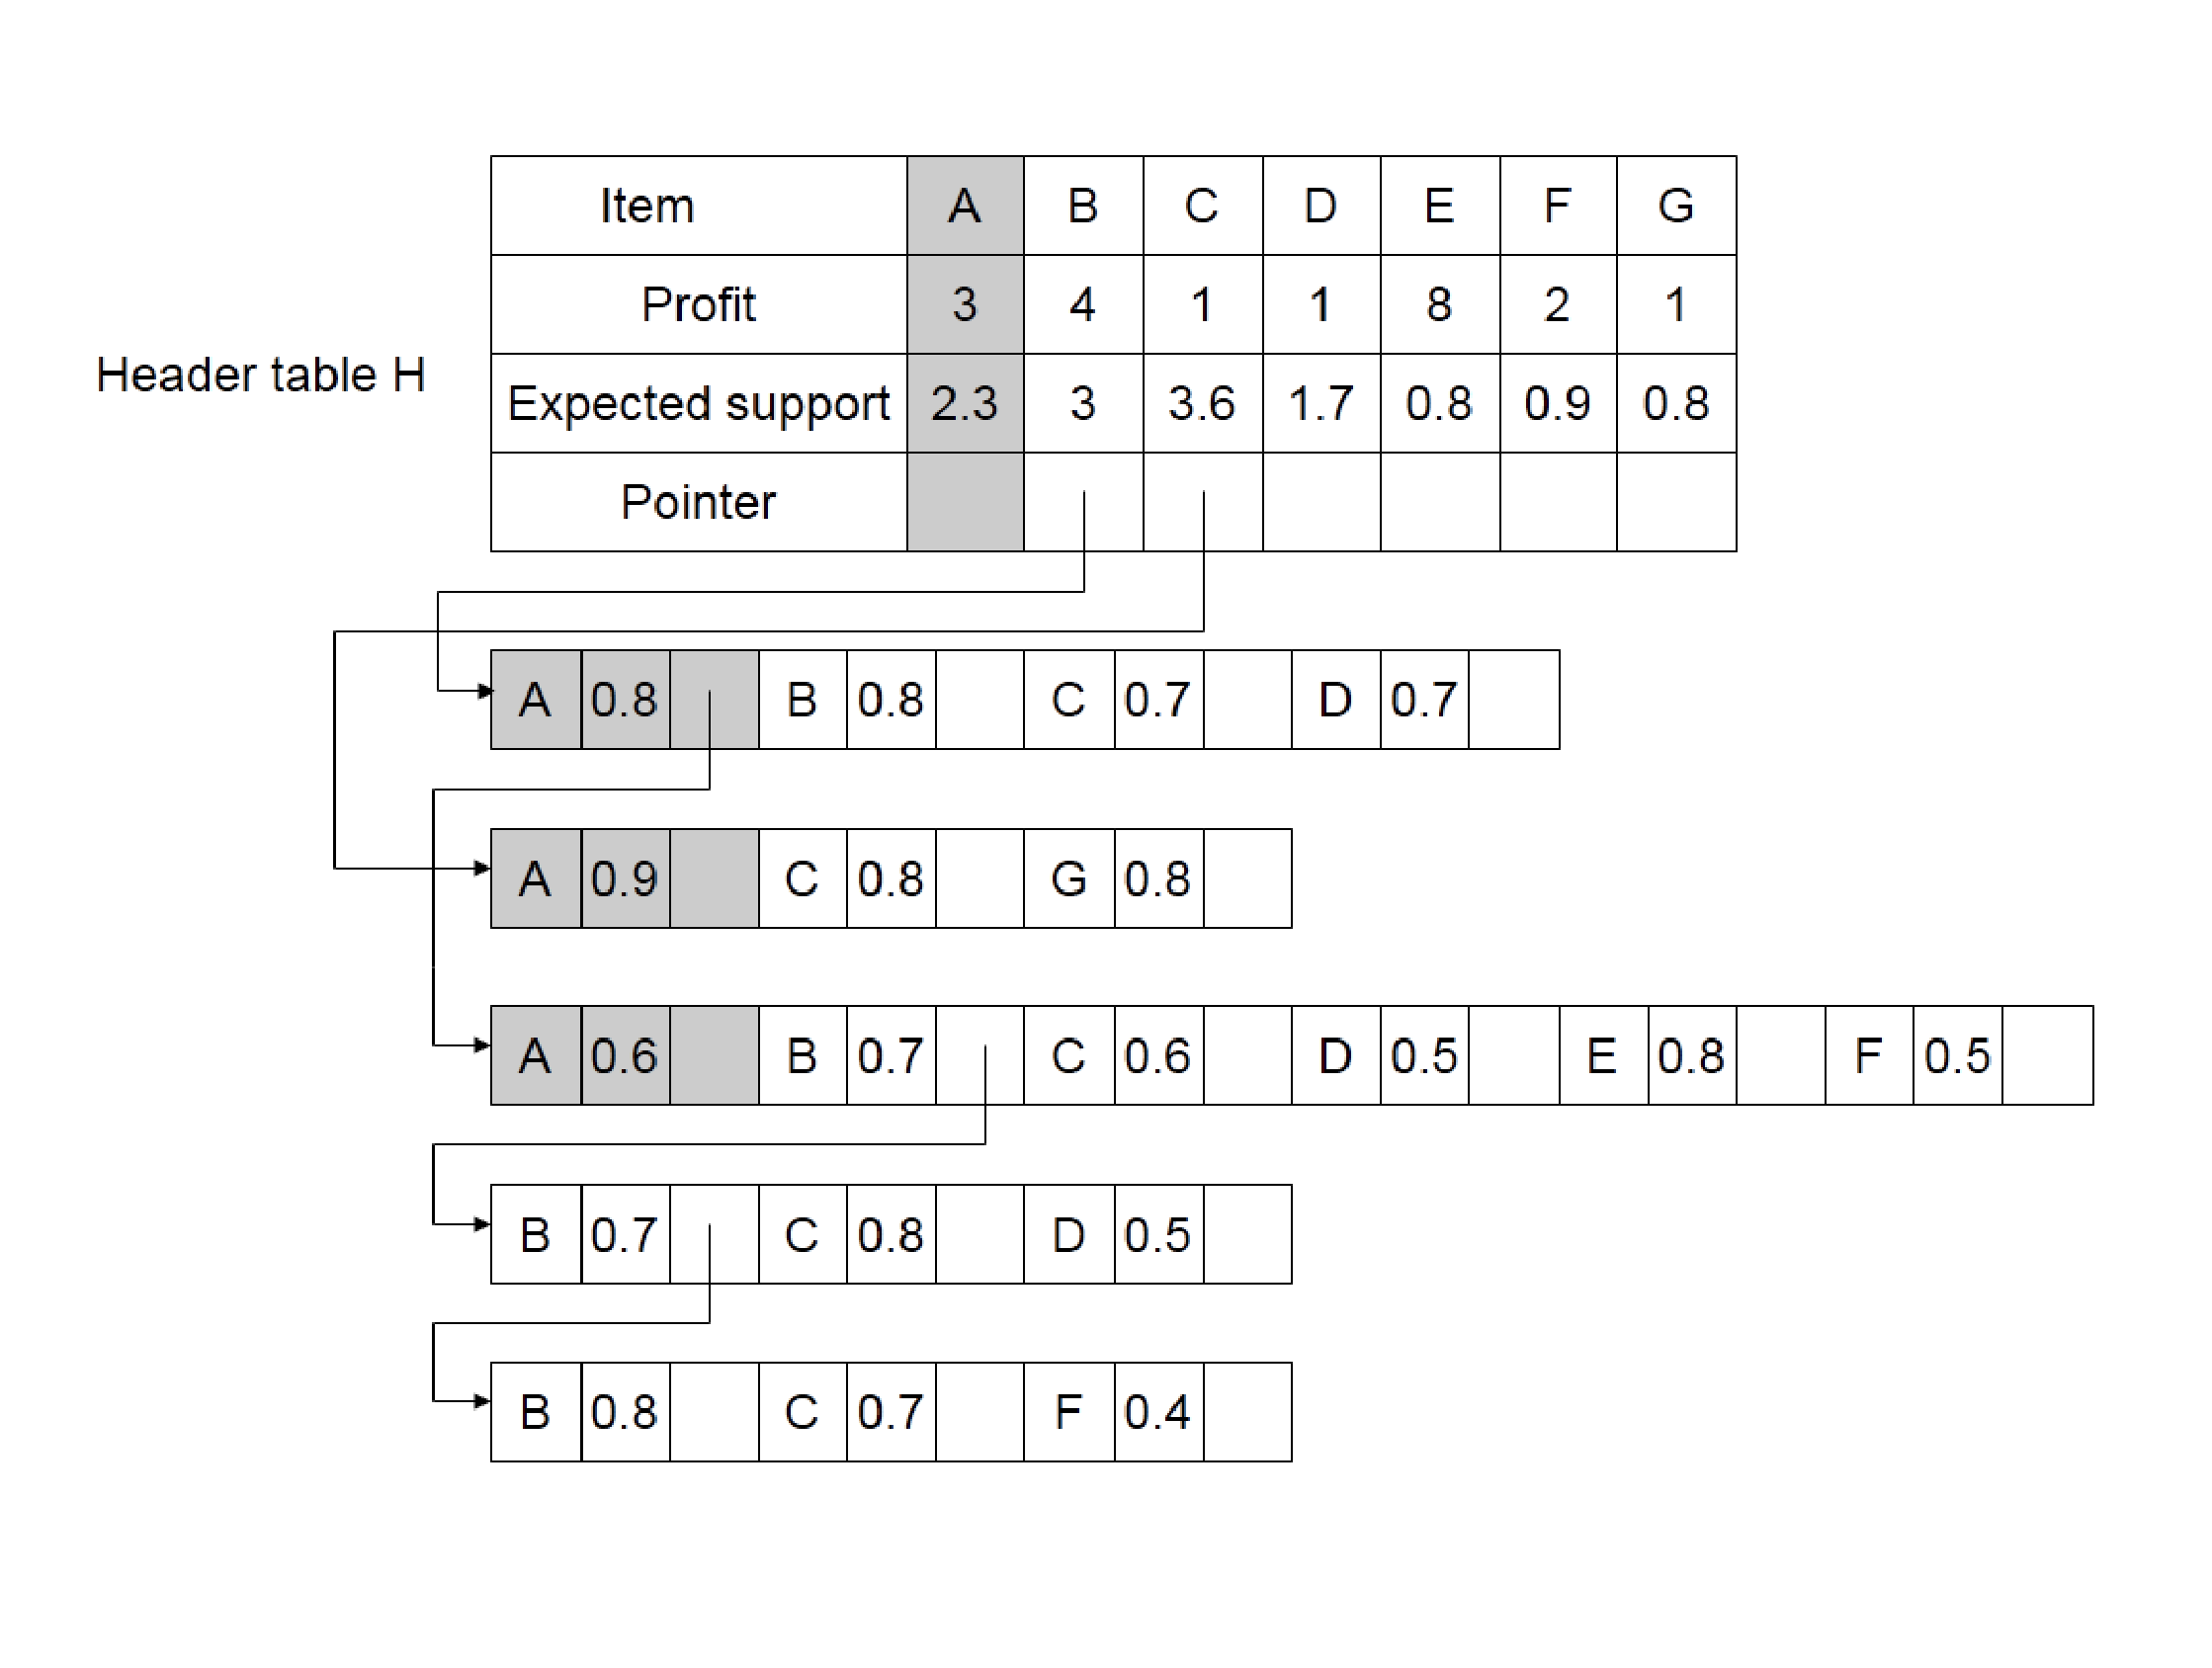
\includegraphics[width=0.23\textwidth]{3.eps}}
  \subfigure{
      \label{fig:memory:sf}
      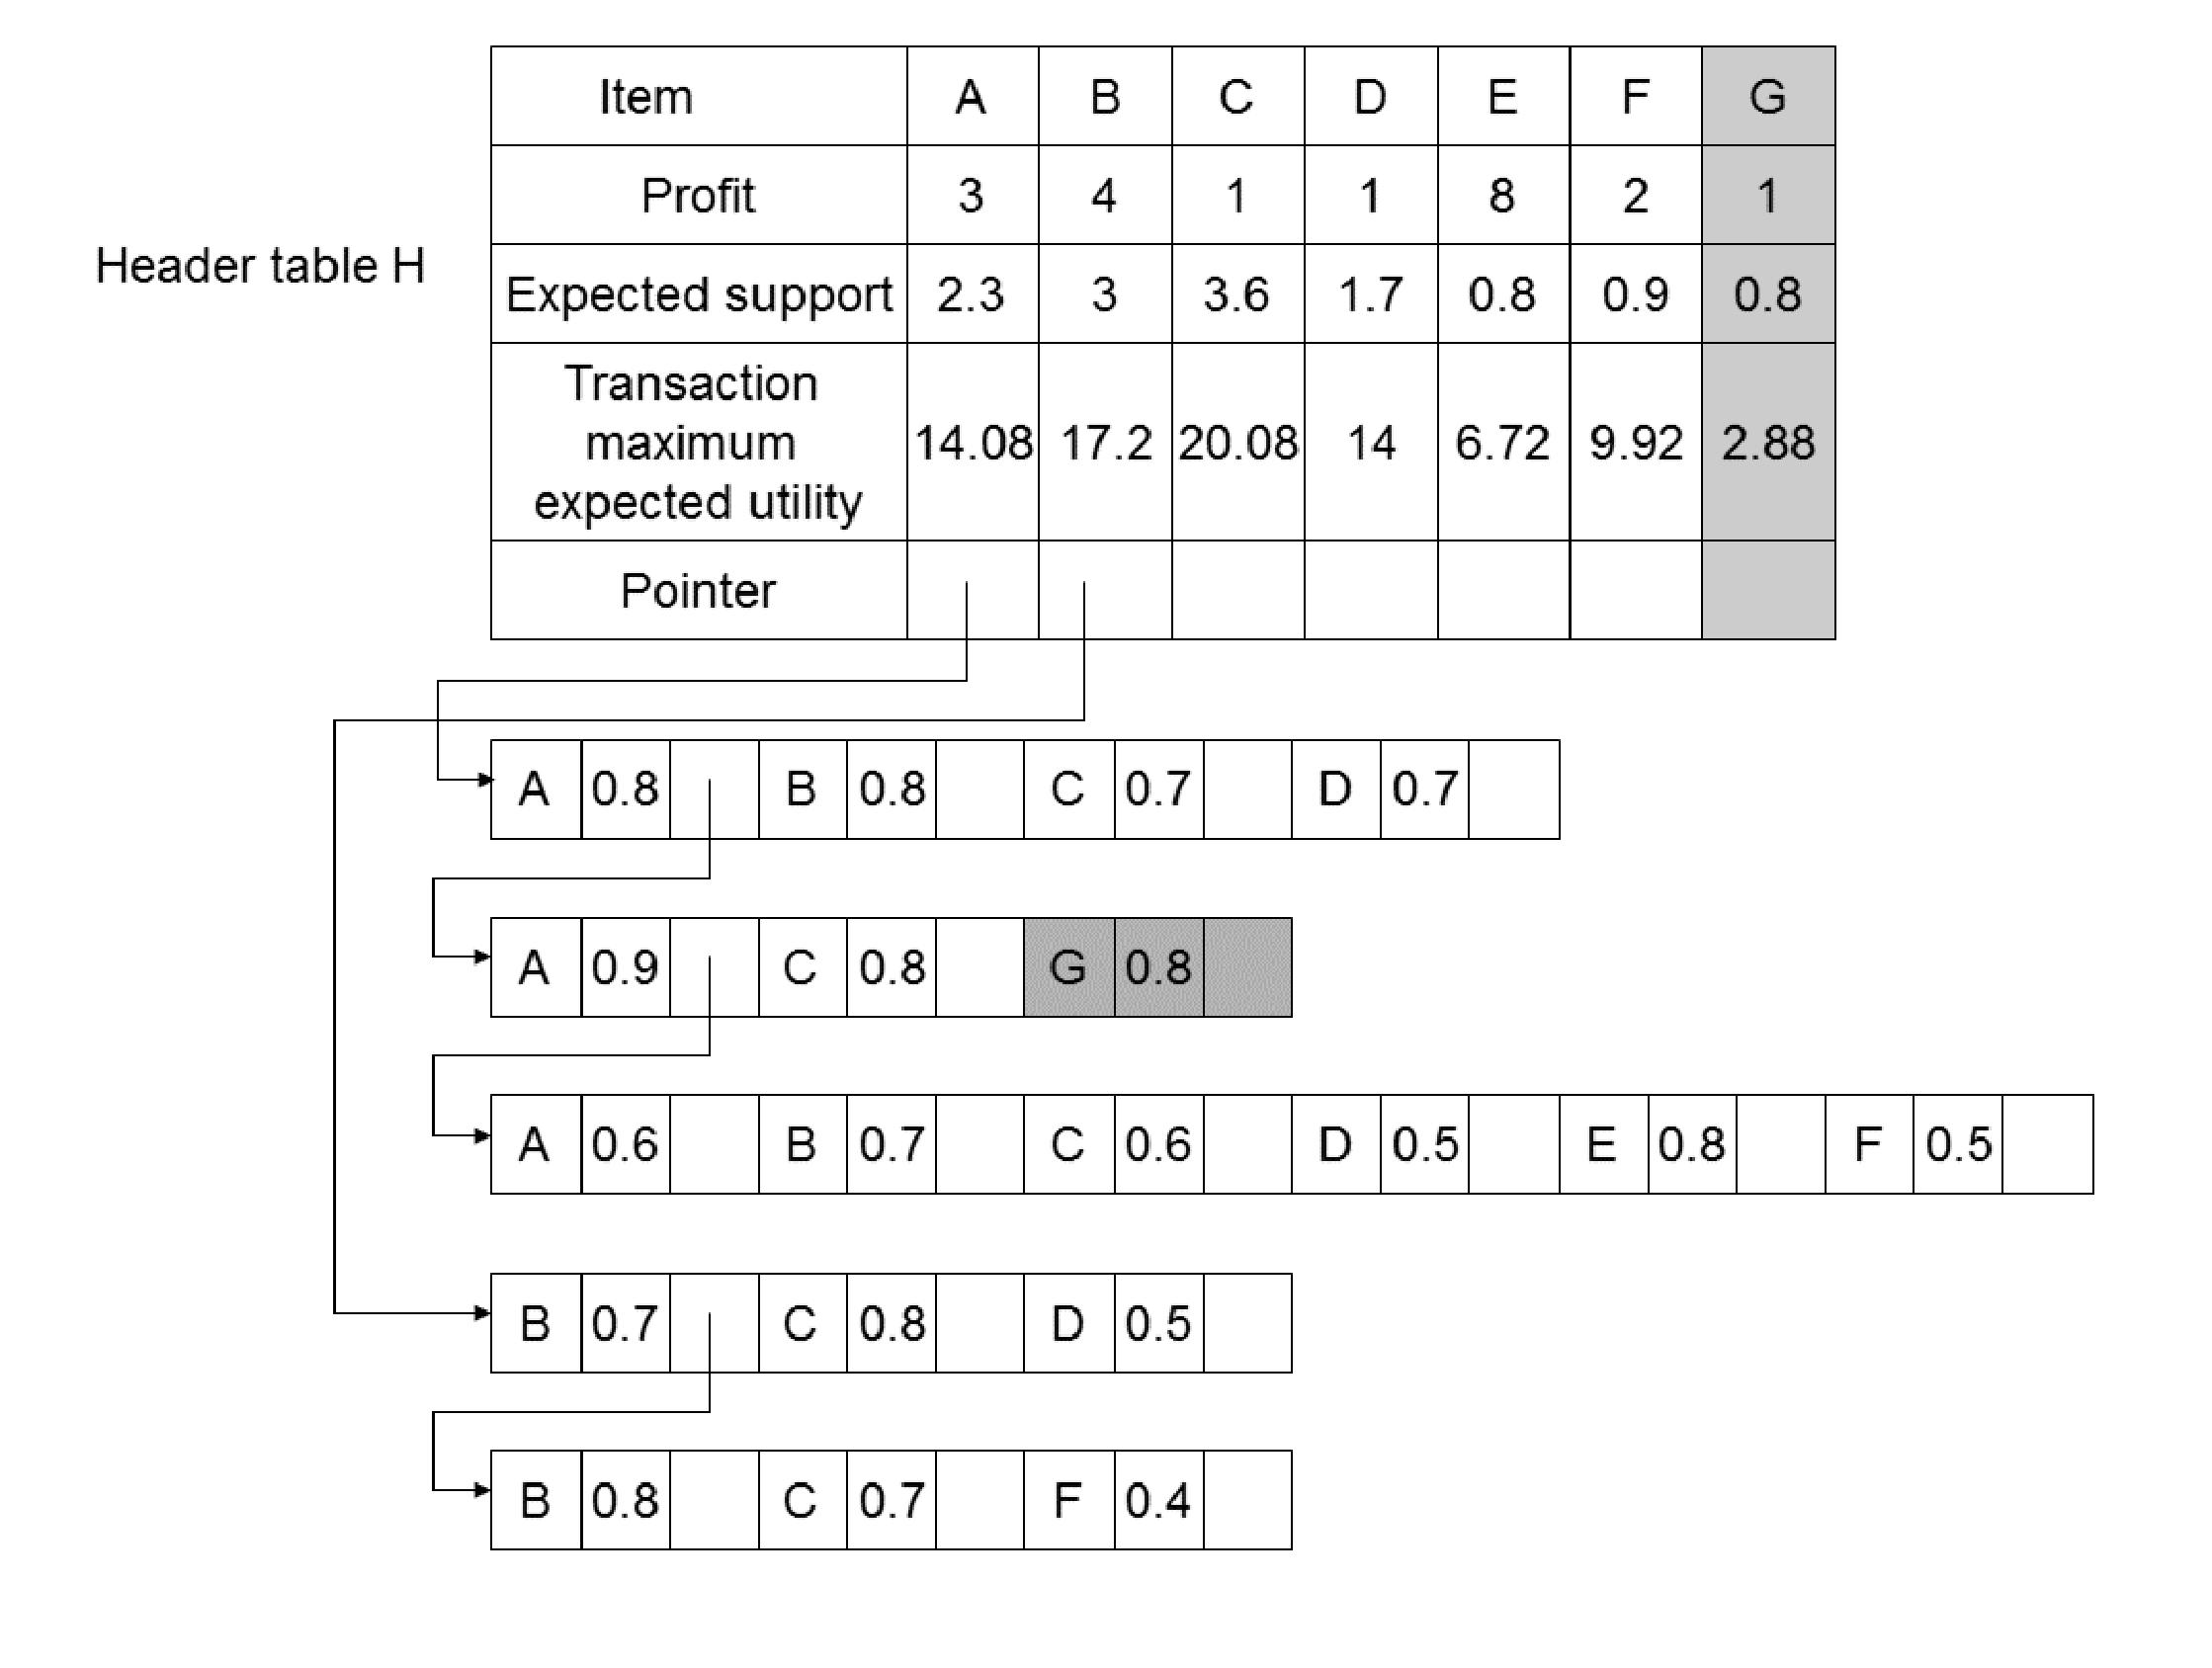
\includegraphics[width=0.23\textwidth]{4.eps}}
\vspace{-0.3cm}
  \caption{Memory consumption under varied MUs}
  \label{fig:time}
\vspace{-0.4cm}
\end{figure}

From Fig.2, it can be clearly seen that the proposed UHUI-apriori algorithm requires less memory compared to the algorithm of direct traversal under varied MUs.

\section{Conclusion And Future Works}
In this paper, a UHUI-apriori algorithm is proposed for mining high utility itemsets over uncertain databases. Different from the algorithm of direct traversal, UHUI-apriori algorithm is based on the TWUDC property. By the evaluation of experiments, UHUI-apriori algorithm is much better than the algorithm of direct traversal in both running time and memory consumption.

Since this is the first work for mining high utility itemsets over uncertain databases, further research issues including dynamic data mining, stream mining, and top-k patterns mining can also be studied. Besides, designing more efficient and condensed structure based on different uncertain models for mining the desired information is also another critical issue in the nearly future.




% conference papers do not normally have an appendix


% use section* for acknowledgement
\section*{Acknowledgment}
This work is supported in part by the National Natural Science Foundation of China (Grant No.61232009).

%The authors would like to thank...





% trigger a \newpage just before the given reference
% number - used to balance the columns on the last page
% adjust value as needed - may need to be readjusted if
% the document is modified later
%\IEEEtriggeratref{8}
% The "triggered" command can be changed if desired:
%\IEEEtriggercmd{\enlargethispage{-5in}}

% references section

% can use a bibliography generated by BibTeX as a .bbl file
% BibTeX documentation can be easily obtained at:
% http://www.ctan.org/tex-archive/biblio/bibtex/contrib/doc/
% The IEEEtran BibTeX style support page is at:
% http://www.michaelshell.org/tex/ieeetran/bibtex/
%\bibliographystyle{IEEEtran}
% argument is your BibTeX string definitions and bibliography database(s)
%\bibliography{IEEEabrv,../bib/paper}
%
% <OR> manually copy in the resultant .bbl file
% set second argument of \begin to the number of references
% (used to reserve space for the reference number labels box)
%\begin{thebibliography}{1}
%
%\bibitem{IEEEhowto:kopka}
%R.~Agrawal, T.~Imieliński, A.~Swami, \emph{Mining association rules between sets of items in large databases}. In SIGMOD’ 1993.
%
%\bibitem{IEEEhowto:kopka}
%R.~Agrawal, R.~Srikant, \emph{Fast algorithms for mining association rules}. In VLDB’ 1994.
%
%\bibitem{IEEEhowto:kopka}
%Y.~Tong, L.~Chen, Y.~Cheng, et al, \emph{Mining frequent itemsets over uncertain databases}. In VLDB’ 12.
%
%\bibitem{IEEEhowto:kopka}
%C.~K.~Chui, B. Kao, E. Hung, \emph{Mining frequent itemsets from uncertain data}. In PAKDD’ 2007.
%
%\bibitem{IEEEhowto:kopka}
%C.~C.~Aggarwal, Y.~Li, J.~Wang, et al, \emph{Frequent pattern mining with uncertain data}. In SIGKDD’ 2009.
%
%\bibitem{IEEEhowto:kopka}
%R.~C.~Chan, Q.~Yang, Y.~D.~Shen, \emph{Mining high utility itemsets}. In ICDM’ 2003.
%
%\bibitem{IEEEhowto:kopka}
%C.~F.~Ahmed, S.~K.~Tanbeer, B.~S.~Jeong, et al, \emph{Efficient tree structures for high utility pattern mining in incremental databases}. IEEE Trans. Knowl. Data Eng. 2013.
%
%\bibitem{IEEEhowto:kopka}
%V.~S.~Tseng, B.~E.~Shie, C.~W.~Wu, et al, \emph{Efficient algorithms for mining high utility itemsets from transactional databases}. IEEE Trans. Knowl. Data Eng. 2013.
%
%\end{thebibliography}

\bibliographystyle{IEEEtran}

\bibliography{utility}


% that's all folks
\end{document}


